\section{Evaluation}
\label{sec: eval}

In this section, we evaluate the following questions regarding Meteor's design.

\begin{itemize}

\item To what extent data locality achieved through LAM decrease job time and bandwidth consumed?
\item What's the improvement in latency when BAWS is used on top of LAM?

\end{itemize}

For our evaluation, we use the Emulab testbed \cite{emulab}. Emulab gives us the ability to configure arbitrary network topologies and link bandwidths. In this initial evaluation, each node in our Emulab topology represents a datacenter and a link connecting two nodes represents a link in the wide-area. 
%In addition to relatively easier and quicker prototyping 
We plan to extend the setup to contain multiple nodes in a cluster as future work.  We have configured our environment in Emulab by installing Spark and its dependencies. Note that Spark requires the data to be stored on a shared filesystem, such as HDFS. To give our system this illusion while ensuring that data is accessed over the traffic-shaped links, we set up NFS servers at each node and disabled client-side caching. Each emulab node has 2GB RAM, and two Intel Xeon 3.00GHz processors.

For data, we use publicly available wikipedia data. The total size of our dataset is 4GB. We chose this size for fast prototyping, considering emulab's status as a highly shared and thus resource-constrained testbed. 
Each node has a split of the total data on its local storage. Our example query, unless otherwise stated, is 
`word count'. The size of each data block is 64MB. Unless otherwise stated, each data point is the mean of three runs.

\subsection{Job Latency and Bandwidth Usage for LAM}
For this experiment, we use a two-cluster `dumbbell' topology with each `cluster' containing two nodes, and
connected to the other cluster with a WAN link. Data is split equally between the two clusters. 
Figure~\ref{fig:job-time-localMap} shows how the job execution time changes as the link bandwidth is varied,  %This is compared against both nodes col-located, i.e., without communication over the WAN. 
with MapReduce/Spark  compared with Location-Aware Map (LAM). 
It clearly shows that the job runtime is very sensitive to the amount of available bandwidth between workers. The Spark runtime is improved by almost 100 secs when the available bandwidth is increased from 5 to 10 Mbps, with it further decreasing as the bandwidth is increased.  
In contrast, LAM achieves significantly better runtime even when the bandwidth is really small. This is expected since data locality is strictly enforced and hence no map input block travels over the WAN link. 
The slight decrease in runtime as the link bandwidth goes up is due to the fact that reduce input still
uses the link due to the all-to-all nature of the reduce phase. 

\begin{figure}[!ht]
\centering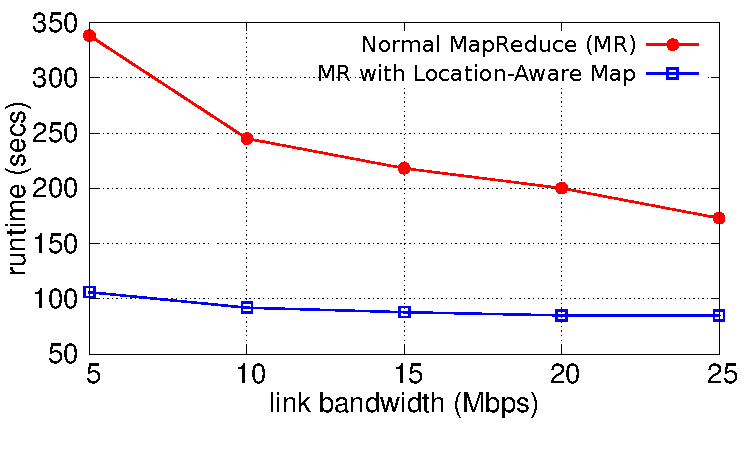
\includegraphics[width=\columnwidth]{figs/job-time-localMap.pdf}
\vspace{-1.2em}
\caption{Spark job execution time increases drastically as the wide area link bandwidth decreases. Latency 
for the Location-Aware Map is significantly better.}
\label{fig:job-time-localMap}
\vspace{.7em}
\end{figure}

\begin{figure}[!ht]
\centering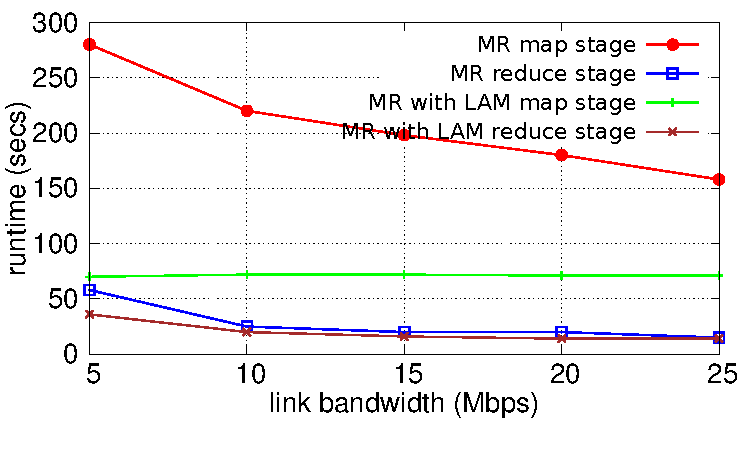
\includegraphics[width=\columnwidth]{figs/stage-time-localMap.pdf}
\vspace{-1.2em}
\caption{Enforcing data locality for the map stage makes map runtime constant no matter the available bandwidth.}
\label{fig:stage-time-localMap}
\vspace{.7em}
\end{figure}

Figure~\ref{fig:stage-time-localMap} splits the runtimes shown in Figure~\ref{fig:stage-time-localMap} into the individual map and reduce stages. It's evident that most of the improvement comes from enforcing strict data locality through LAM and hence make the map runtime independent of the link bandwidth. 

\subsection{Job Latency for BAWS}

Two measure the effect of Bandwidth-Aware Work Stealing, we use a topology containing three nodes with every pair of nodes connected together.  

\begin{figure}[!ht]
\centering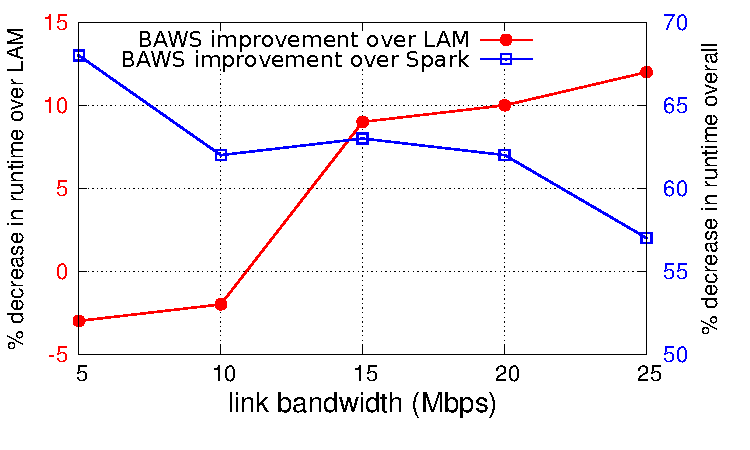
\includegraphics[width=\columnwidth]{figs/baws.pdf}
\vspace{-1.2em}
\caption{Enforcing data locality for the map stage makes map runtime constant no matter the available bandwidth.}
\label{fig:stage-time-localMap}
\vspace{.7em}
\end{figure}


